\vspace{0.5cm}
\subsubsection{Résultats pour un Débit Physique de 125 Mbit/s}
\begin{figure}[H]
    \centering
    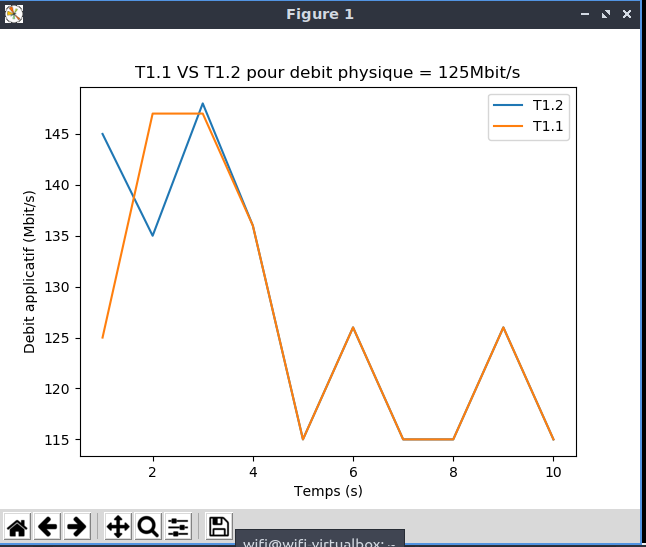
\includegraphics[width=1\textwidth]{./images/T1vsT2pour125.png}
    \caption{Courbe de Test1 VS Test2 pour debit physique = 125Mbit/s}
    \label{fig:exemple}
\end{figure}

\textbf{Analyse :}\\
\textbf{Comportement Initial :} T1.2 affiche un débit initial plus élevé (environ 145 Mbit/s) par rapport à T1.1, qui démarre autour de 125 Mbit/s.\\
\textbf{Stabilité et Fluctuations :} Les deux configurations atteignent un pic de débit entre 2 et 3 secondes,  mais ensuite, elles diminuent pour prendre des valeurs inférieurs à 125 Mbit/s\\
\textbf{Conclusion (125 Mbit/s) :}  Les deux configurations commencent de manière différente, mais après un certain temps, les deux configurations finissent par se rapprocher en termes de comportement, montrant une instabilité similaire.

\subsubsection{Résultats pour un Débit Physique de 625 Mbit/s}
\begin{figure}[H]
    \centering
    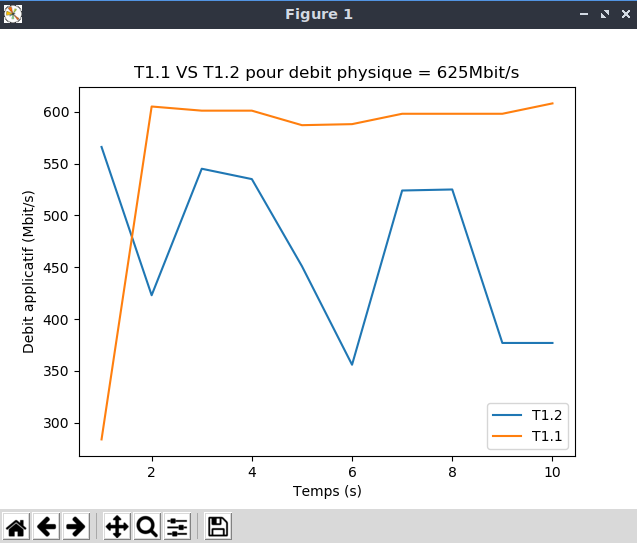
\includegraphics[width=1\textwidth]{./images/T1vsT2pour625.png}
    \caption{Courbe de Test1 VS Test2 pour debit physique = 625Mbit/s}
    \label{fig:exemple}
\end{figure}

\textbf{Analyse :}\\
\textbf{Comportement Initial :} T1.1 atteint rapidement environ 600 Mbit/s et reste stable, tandis que T1.2 montre des fluctuations initiales, atteignant environ 550 Mbit/s.\\
\textbf{Stabilité et Consistance :} T1.1 est stable et proche de la limite physique, tandis que T1.2 est instable, avec des variations importantes.\\
\textbf{Conclusion (625 Mbit/s) :} Le lien direct (T1.1) offre une performance supérieure, avec un débit plus stable.

\subsubsection{Interprétation des Résultats pour un Débit Physique de 2,5 Gbit/s}
\begin{figure}[H]
    \centering
    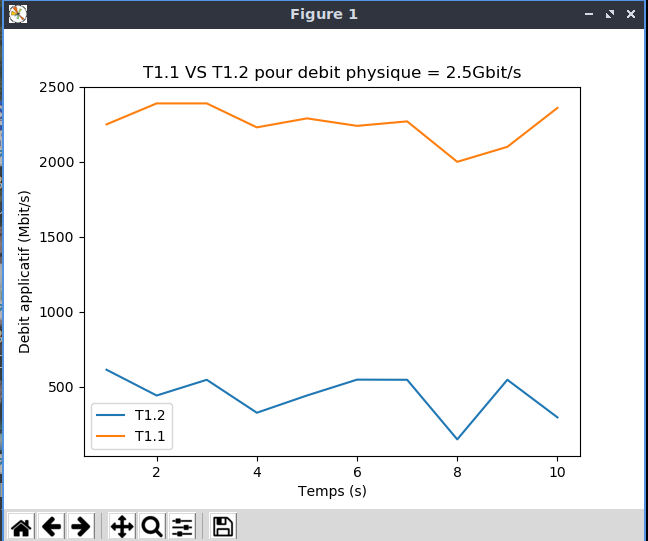
\includegraphics[width=1\textwidth]{./images/T1vsT2pour2500.png}
    \caption{Courbe de Test1 VS Test2 pour debit physique = 2.5Gbit/s}
    \label{fig:exemple}
\end{figure}

\textbf{Analyse :}\\
\textbf{Performance du Lien Direct (T1.1) :}Le débit mesuré est d'environ 2,4 Gbit/s, indiquant une communication efficace et proche de la capacité maximale du lien.\\
\textbf{Performance avec le Switch (T1.2) :} Le débit fluctue autour de 600 Mbit/s, en raison de la limitation imposée par le débit physique entre le switch et l'hôte, d'éventuels goulots d'étranglement et des processus de traitement dans le switch\\
\textbf{Conclusion (2,5 Gbit/s) :} Le lien direct est plus performant à des débits élevés, étant donné que l'ajout d'un switch entraîne une dégradation notable du débit.
\newpage
\subsubsection{Interprétation Générale: }
\textbf{Impact de la Topologie du Réseau :}\\
L’ajout d’un switch avec une limitation de débit modifie fondamentalement la capacité du réseau à transmettre un débit élevé.L’absence de goulot d’étranglement dans le Test 1 permet d’atteindre un débit applicatif optimal, alors que la présence du switch dans le Test 2 empêche l’hôte h2 de bénéficier d’une augmentation du débit physique.

\textbf{Lien Direct (T1.1) :} Offre une meilleure performance, minimisant les latences et maximisant l'utilisation du débit physique.

\textbf{Switch (T1.2) :} Introduit une surcharge, réduisant la performance, surtout à des débits élevés.\\

Pour des applications nécessitant un débit élevé et constant, une connexion directe est préférable. L'utilisation d'un switch est recommandée pour des scénarios nécessitant flexibilité et expansion du réseau, bien qu'elle puisse entraîner des baisses de performance. En résumé, le choix de la topologie doit être basé sur les exigences de l'application, en équilibrant performance et flexibilité.
\section {Conclusion: }
Les résultats des tests réalisés mettent en évidence l'impact significatif de la configuration du réseau et des équipements intermédiaires sur le débit applicatif. Lorsqu'il n'y a pas de limitations causées par des éléments intermédiaires tels que des switches, l'augmentation du débit physique se traduit directement par une amélioration du débit applicatif. Cela suggère que, dans des conditions idéales, le débit applicatif peut évoluer de manière linéaire avec le débit physique, permettant ainsi d’optimiser les performances du réseau. Cependant, l'introduction de restrictions intermediaires, notamment par la présence d'un switch avec un débit limité, peut entraîner une saturation du débit applicatif. Dans ce cas, bien que le débit physique sur d'autres segments du réseau soit augmenté, cela n’a que peu ou pas d'effet sur le débit applicatif, qui atteint rapidement un plafond. Ce phénomène souligne l'importance de la gestion adéquate de la capacité des équipements intermédiaires, afin de maximiser l'efficacité du réseau et d’éviter toute dégradation des performances due à des limitations imprévues.
